% Title Page
\begin{titlepage}
    \centering
    \vspace*{2cm}

    % Main title
    {\Huge\bfseries\scshape Wayland\par}
    \vspace{1cm}
    {\Large A Complete Guide to Modern Display Server Architecture\par}
    \vspace{2cm}

    % Subtitle
    {\large\itshape Philosophy, Protocol, and Practice\par}
    \vspace{3cm}

    % Visual element - could be replaced with actual graphics
    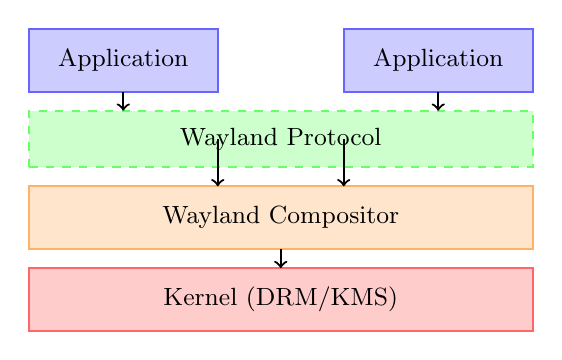
\begin{tikzpicture}[scale=0.8]
        % Draw a simplified display server architecture
        % Application layer
        \draw[fill=blue!20, draw=blue!60, thick] (-4,3) rectangle (-1,4);
        \node at (-2.5,3.5) {\small Application};

        \draw[fill=blue!20, draw=blue!60, thick] (1,3) rectangle (4,4);
        \node at (2.5,3.5) {\small Application};

        % Wayland Protocol
        \draw[fill=green!20, draw=green!60, thick, dashed] (-4,1.8) rectangle (4,2.7);
        \node at (0,2.25) {\small Wayland Protocol};

        % Compositor
        \draw[fill=orange!20, draw=orange!60, thick] (-4,0.5) rectangle (4,1.5);
        \node at (0,1) {\small Wayland Compositor};

        % Kernel/Hardware
        \draw[fill=red!20, draw=red!60, thick] (-4,-0.8) rectangle (4,0.2);
        \node at (0,-0.3) {\small Kernel (DRM/KMS)};

        % Arrows showing communication
        \draw[->, thick] (-2.5,3) -- (-2.5,2.7);
        \draw[->, thick] (2.5,3) -- (2.5,2.7);
        \draw[->, thick] (-1,2.25) -- (-1,1.5);
        \draw[->, thick] (1,2.25) -- (1,1.5);
        \draw[->, thick] (0,0.5) -- (0,0.2);
    \end{tikzpicture}

    \vfill

    % Author
    {\Large\itshape 1ay1\par}
    \vspace{0.5cm}
    {\small \url{https://github.com/1ay1/wayland_book}\par}
    \vspace{1cm}

    % Publication info
    {\large Version 1.0\par}
    {\large \today\par}

    \vspace{1cm}

    % Tagline
    {\small\itshape Understanding the future of Linux graphics, one protocol at a time.\par}

\end{titlepage}

\clearpage
